% =====================================================================
%  OELLM — Observation of Earth Large Language Model
%  Graduation-project defense pitch (~8 min, ~9 slides)
%  Theme: metropolis, recoloured to the OELLM poster palette.
%
%  Compile:  pdflatex slides.tex   (or: latexmk -pdf slides.tex)
%  Needs the 'metropolis' beamer theme:
%     - TeX Live:  tlmgr install beamertheme-metropolis
%     - or via:    \usepackage{pgfplots} ; sometimes already present
%  If metropolis is unavailable, replace \usetheme{metropolis} with
%  \usetheme{default} — the colour definitions below still apply.
% =====================================================================
\documentclass[aspectratio=169, 11pt]{beamer}

\usetheme{metropolis}
\usepackage{booktabs}
\usepackage{graphicx}
\usepackage{xcolor}
\usepackage{tikz}
\usepackage{colortbl}
\usepackage{appendixnumberbeamer}
\usetikzlibrary{positioning, arrows.meta}

% ---------- OELLM poster palette --------------------------------------
\definecolor{oellmblue}{HTML}{0E3B6B}
\definecolor{oellmsky}{HTML}{1F77B4}
\definecolor{oellmorange}{HTML}{E07B19}
\definecolor{oellmgreen}{HTML}{2CA02C}
\definecolor{oellmred}{HTML}{C0392B}
\definecolor{oellmgold}{HTML}{D4A017}
\definecolor{paperbg}{HTML}{F7F4EE}
\definecolor{soft}{HTML}{443F3A}

% Recolour metropolis to the poster identity
\setbeamercolor{normal text}{fg=soft, bg=white}
\setbeamercolor{alerted text}{fg=oellmorange}
\setbeamercolor{example text}{fg=oellmgreen}
\setbeamercolor{frametitle}{bg=oellmblue, fg=white}
\setbeamercolor{title separator}{fg=oellmorange}
\setbeamercolor{progress bar}{fg=oellmorange}
\setbeamercolor{progress bar in head/foot}{fg=oellmorange}
\setbeamercolor{progress bar in section page}{fg=oellmorange}

% shorthands
\newcommand{\good}[1]{\textcolor{oellmgreen}{\textbf{#1}}}
\newcommand{\bad}[1]{\textcolor{oellmred}{\textbf{#1}}}
\newcommand{\hi}[1]{\textcolor{oellmorange}{\textbf{#1}}}
\newcommand{\blue}[1]{\textcolor{oellmblue}{\textbf{#1}}}

\setbeamertemplate{frame numbering}[fraction]
\setbeamerfont{frametitle}{size=\large}

% ---------- title ----------
\title{OELLM}
\subtitle{Observation of Earth Large Language Model\\
\normalsize A Vision--Language Model for Urban Understanding \&\\ Cross-View Geolocalisation}
\author{Ezel Bayraktar \and Alperen Demirci \and Mukhamediyar Amanzhol \and Adam Sattout}
\institute{Hacettepe University, Computer Engineering --- BBM479/480\\
Supervisor: Prof.\ Dr.\ Mehmet Erkut Erdem}
\date{2026}

\begin{document}

% =====================================================================
% 1 — TITLE
% =====================================================================
{
\setbeamercolor{background canvas}{bg=oellmblue}
\setbeamercolor{normal text}{fg=white}
\setbeamercolor{title}{fg=white}
\setbeamercolor{subtitle}{fg=paperbg}
\setbeamercolor{author}{fg=paperbg}
\setbeamercolor{institute}{fg=paperbg}
\setbeamercolor{date}{fg=paperbg}
\begin{frame}
  \titlepage
  \vspace{-1.5em}
  \hfill{\footnotesize\textcolor{oellmorange}{\textbf{Qwen3.5-4B-VL}}\;$\cdot$\; 40 cities \;$\cdot$\; OpenStreetMap-grounded}
\end{frame}
}

% =====================================================================
% 2 — THE PROBLEM
% =====================================================================
\begin{frame}{The problem: VLMs can't really ``read'' a place}
\begin{columns}[T]
\begin{column}{0.56\textwidth}
  \small
  Vision--Language Models are tested on web images, not on geography. Two abilities stay unmeasured:
  \vspace{0.4em}
  \begin{itemize}
    \item \blue{Urban understanding} --- land use, building stock, transit, green space from one location.
    \item \blue{Cross-view geolocalisation} --- do this \emph{satellite} view and this \emph{street} view show the same place? From which direction?
  \end{itemize}
  \vspace{0.5em}
  \begin{block}{The trap}
  \alert{Unimodal shortcut learning}: the model answers from a text prior or one image --- never fusing the two views.
  \end{block}
\end{column}
\begin{column}{0.42\textwidth}
  \centering
  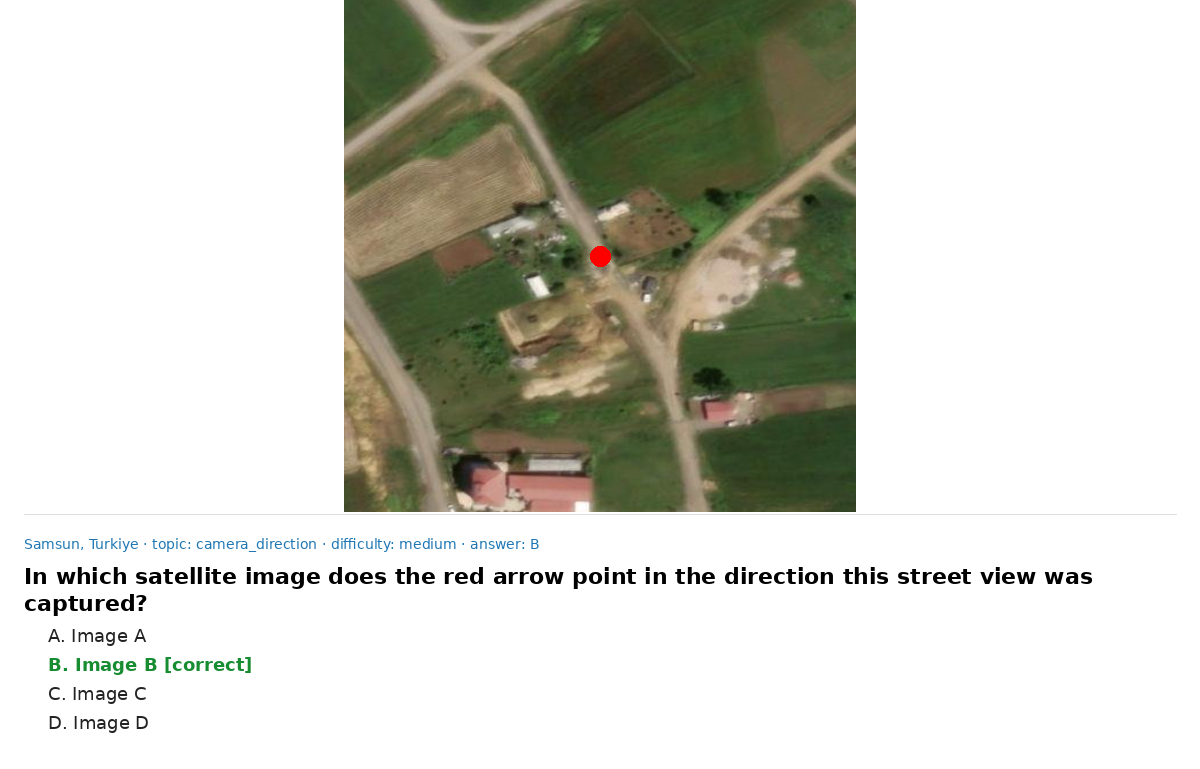
\includegraphics[width=\linewidth]{figures/ex_camera_direction.png}\\
  {\footnotesize\textcolor{soft}{One satellite tile \,$+$\, four street views per location.}}
\end{column}
\end{columns}
\end{frame}

% =====================================================================
% 3 — THE DATASET / PIPELINE
% =====================================================================
\begin{frame}{Our answer: a zero-hallucination, OSM-grounded dataset}
\centering
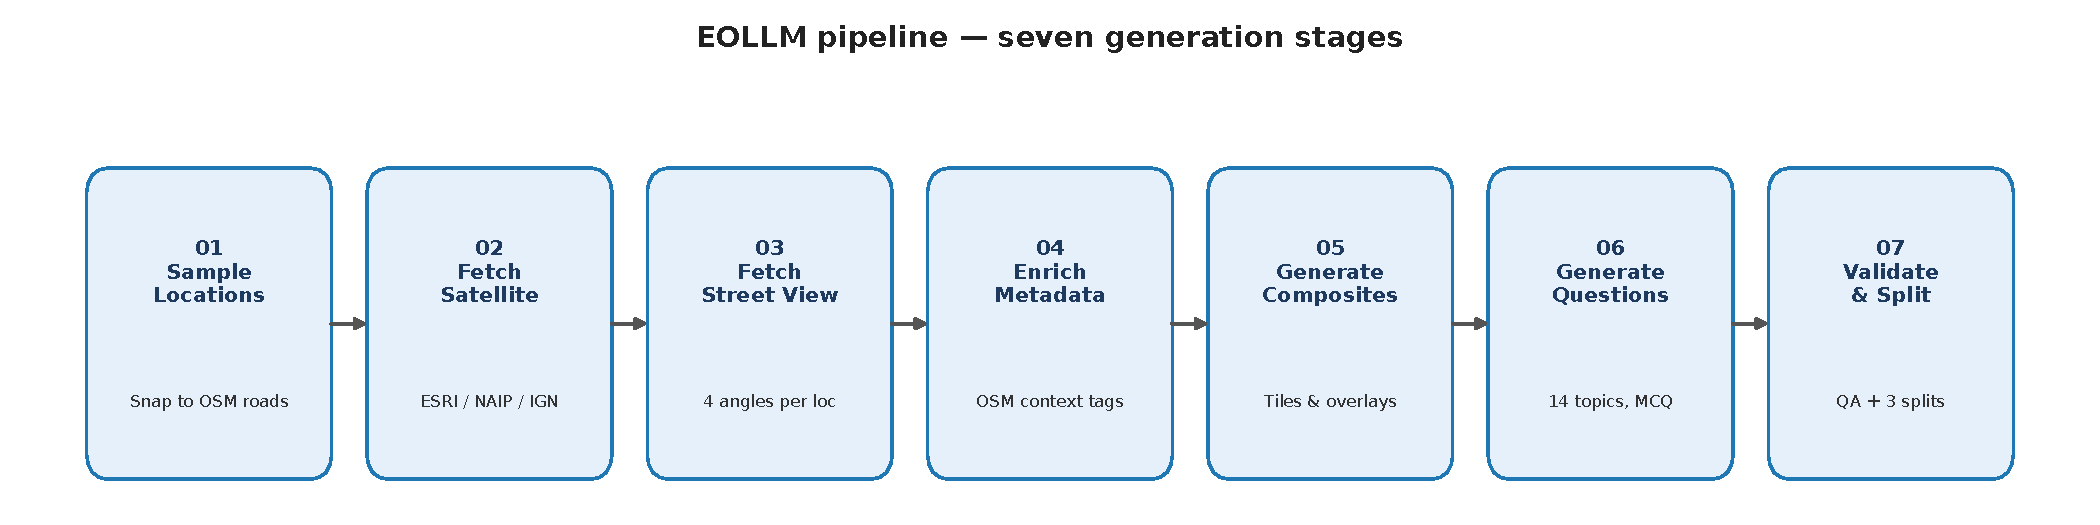
\includegraphics[width=0.94\linewidth]{figures/pipeline.pdf}
\vspace{0.2em}
\begin{columns}[T]
\begin{column}{0.5\textwidth}
\scriptsize
\begin{itemize}
  \item Every answer derived \blue{deterministically from OpenStreetMap} --- no annotators, bit-exact reproducible.
  \item \blue{40 cities}, 32 countries, 6 continents.
\end{itemize}
\end{column}
\begin{column}{0.5\textwidth}
\scriptsize
\begin{itemize}
  \item \blue{39{,}155} question records over \blue{4{,}168} locations.
  \item \blue{14 task types} $\to$ urban understanding $+$ cross-view geometry.
\end{itemize}
\end{column}
\end{columns}
\end{frame}

% =====================================================================
% 4 — METHOD
% =====================================================================
\begin{frame}{Method: a compact model, parameter-efficient tuning}
\begin{columns}[T]
\begin{column}{0.52\textwidth}
  \textbf{Model.} Fine-tune \blue{Qwen3.5-4B-VL} with \blue{LoRA} (vision $+$ language, all-linear), bf16, on a single RTX PRO 6000.
  \vspace{0.5em}

  \textbf{Eval.} Strict \blue{greedy decoding}, deterministic, scored against per-topic \emph{random} and \emph{majority} baselines --- not just chance.
\end{column}
\begin{column}{0.46\textwidth}
  \textbf{Three splits, one taxonomy:}
  \vspace{0.4em}
  \footnotesize
  \begin{tabular}{@{}lll@{}}
  \toprule
  \textbf{Split} & \textbf{Train} & \textbf{Tests} \\
  \midrule
  \textcolor{oellmsky}{per\_city}    & 26{,}931 & new locations \\
  \textcolor{oellmorange}{seen\_unseen} & 26{,}963 & 8 held-out cities \\
  \textcolor{oellmred}{benchmark}   & --- & disjoint, held-out \\
  \bottomrule
  \end{tabular}
  \vspace{0.6em}
  \scriptsize\textcolor{soft}{\textsf{seen\_unseen} is the honest test of geographic generalisation.}
\end{column}
\end{columns}
\end{frame}

% =====================================================================
% 5 — HEADLINE RESULT
% =====================================================================
\begin{frame}{Result: a 4B model beats six open VLMs}
\centering
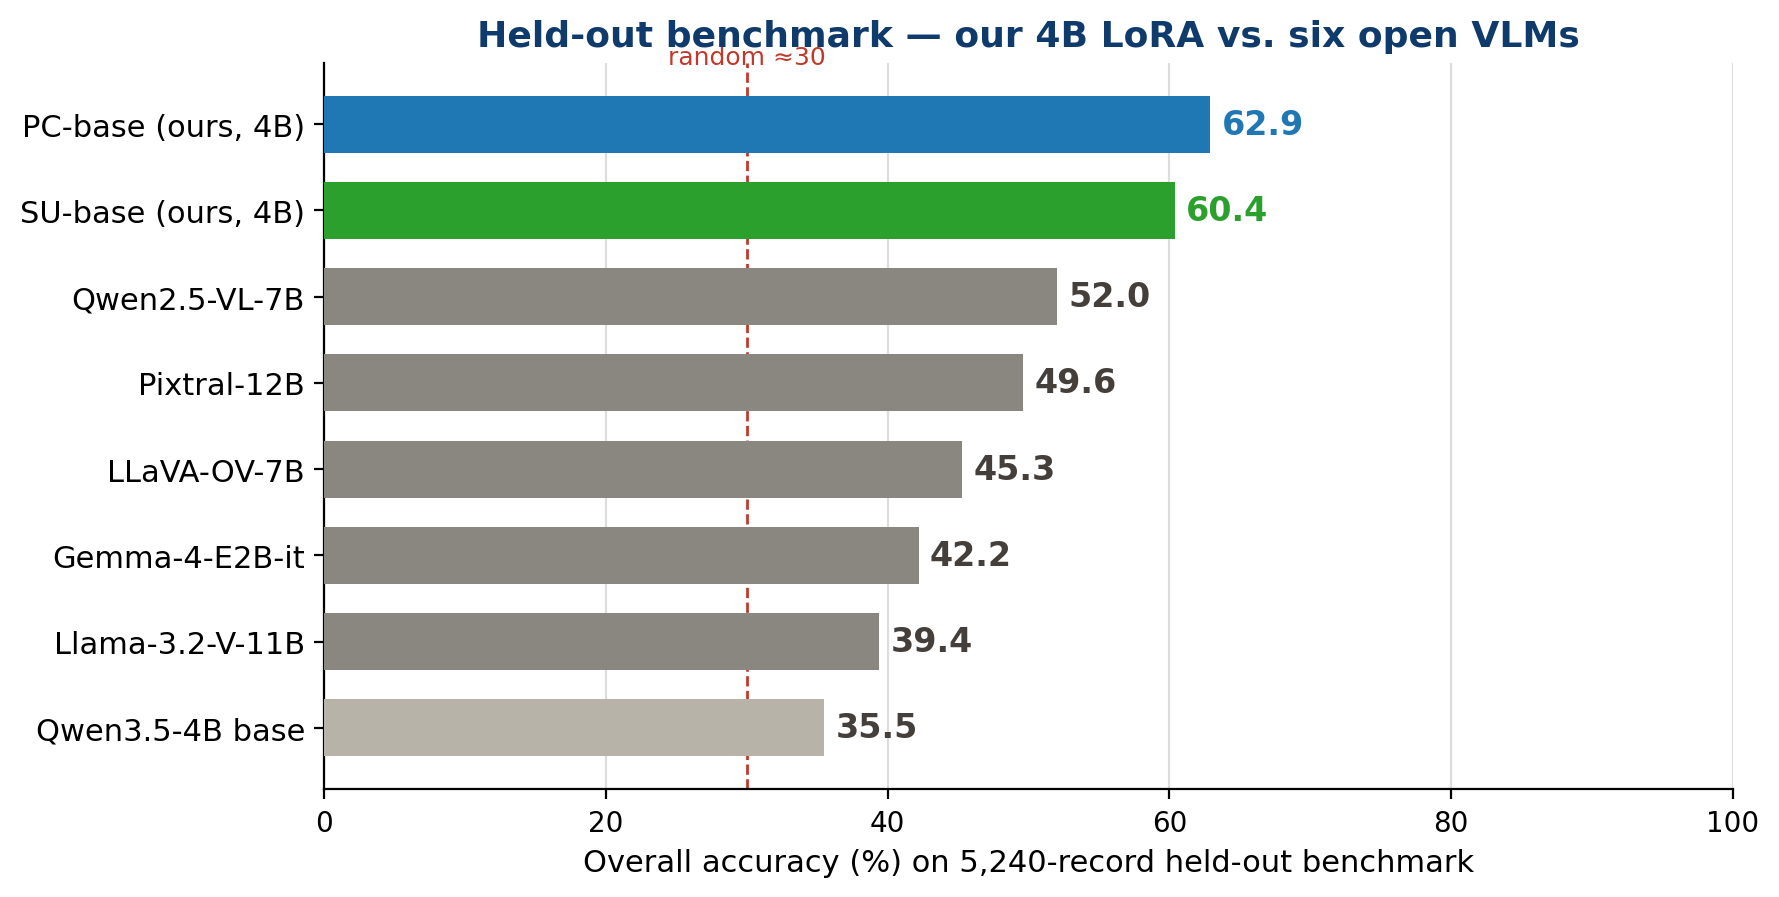
\includegraphics[height=0.74\textheight]{figures/bench_bars.png}\\
{\footnotesize\textcolor{soft}{5{,}240-record held-out benchmark $\cdot$ identical greedy protocol.
Our \textcolor{oellmsky}{\textbf{PC-base}} and \textcolor{oellmgreen}{\textbf{SU-base}} (4B) lead models up to \textbf{3$\times$ larger}.}}
\end{frame}

% =====================================================================
% 6 — THE PAIRED STORY (generalisation)
% =====================================================================
\begin{frame}{The real finding: the skill transfers across cities}
\begin{columns}[T]
\begin{column}{0.46\textwidth}
  \begin{itemize}
    \item \textcolor{oellmsky}{\textbf{PC-base}} (seen cities): \good{62.9\%}
    \item \textcolor{oellmgreen}{\textbf{SU-base}} (8 cities fully held out): \good{60.4\%}
  \end{itemize}
  \vspace{0.6em}
  \begin{alertblock}{Only a 2.5-point gap}
  Holding out \emph{entire cities} costs almost nothing --- the model learns \blue{transferable urban structure}, not memorised places.
  \end{alertblock}
\end{column}
\begin{column}{0.52\textwidth}
  \centering
  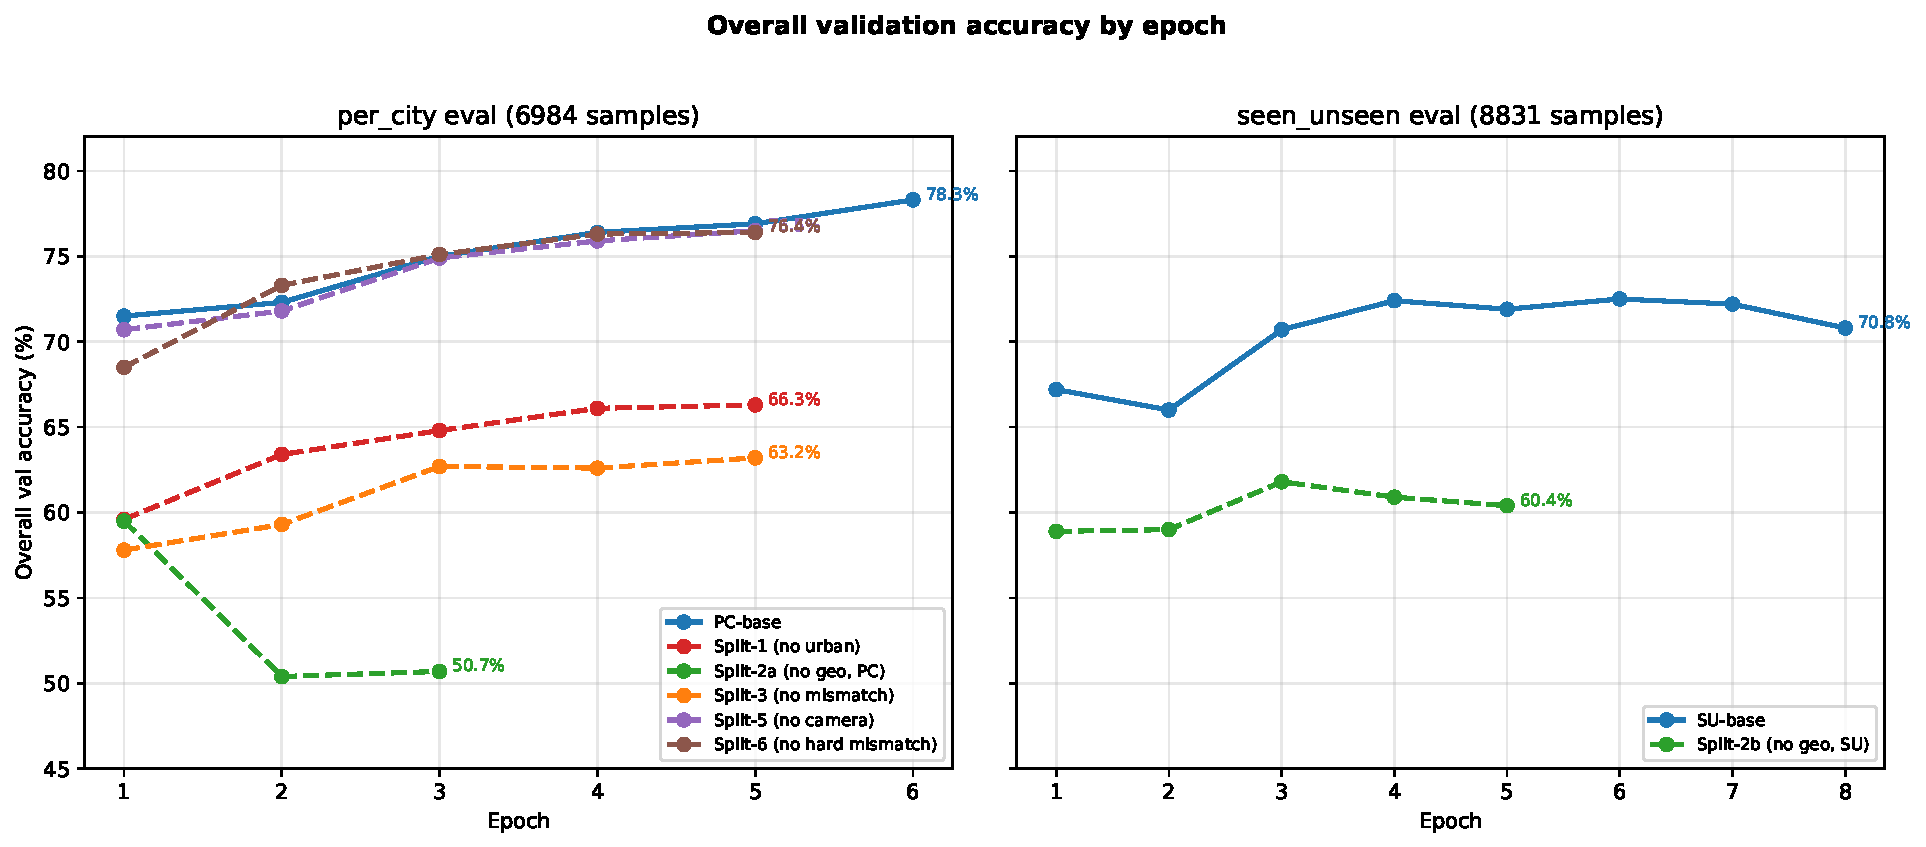
\includegraphics[width=\linewidth]{figures/training_curves.pdf}\\
  {\scriptsize\textcolor{soft}{Validation accuracy by epoch: per-city (left) vs.\ cross-city (right).}}
\end{column}
\end{columns}
\end{frame}

% =====================================================================
% 7 — ABLATIONS: TRANSFER LADDER
% =====================================================================
\begin{frame}{Ablations: which abilities transfer, which don't}
\begin{columns}[T]
\begin{column}{0.5\textwidth}
  \centering
  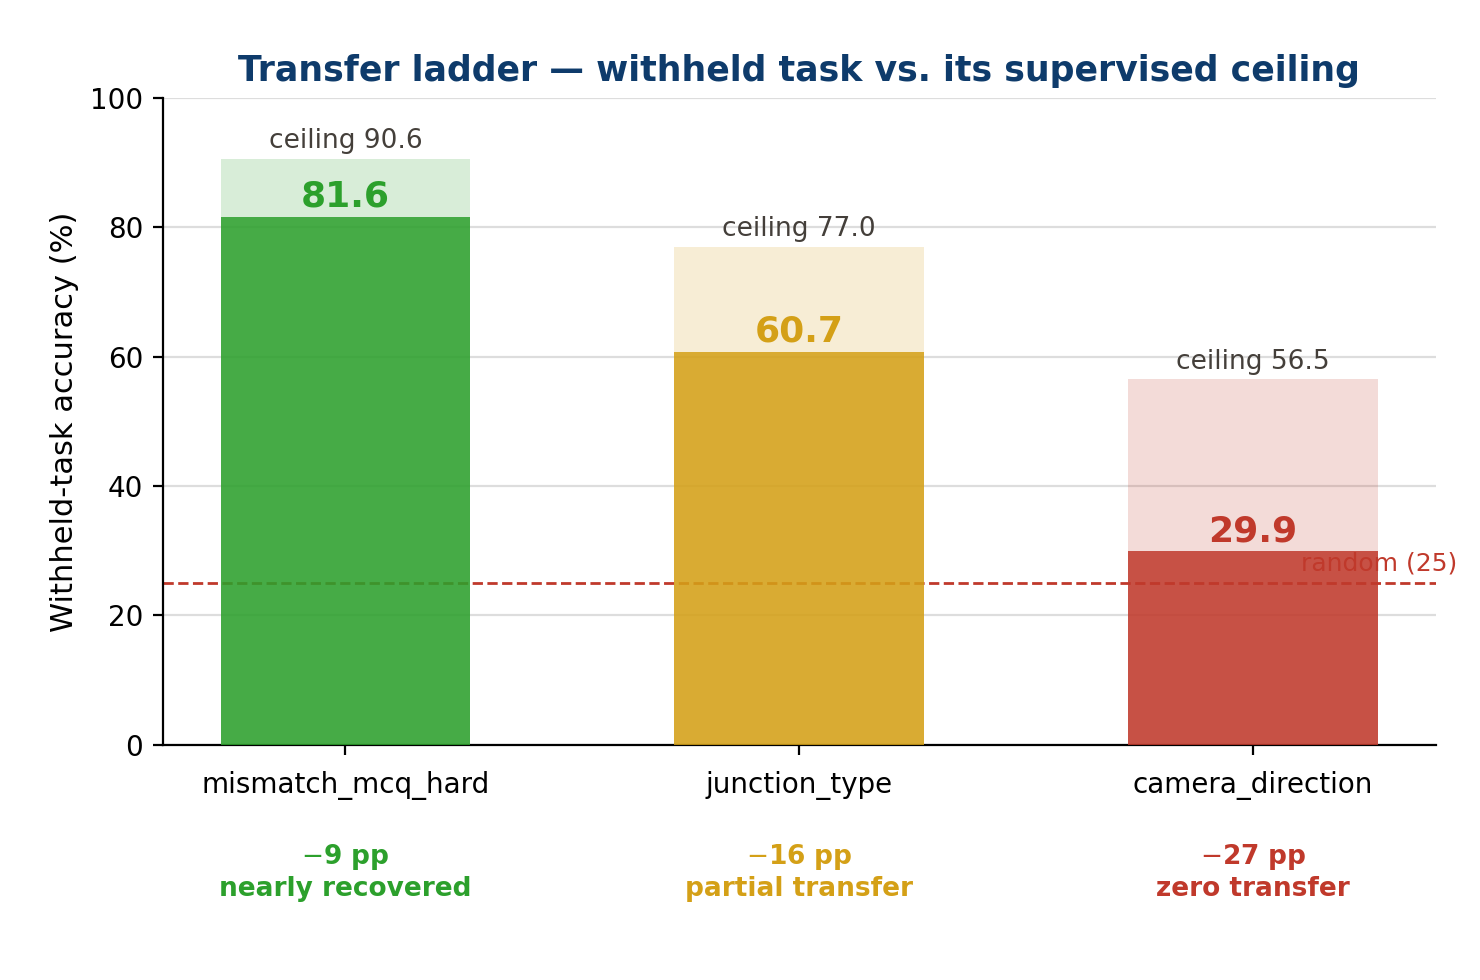
\includegraphics[width=\linewidth]{figures/transfer_ladder.png}
\end{column}
\begin{column}{0.48\textwidth}
  \small
  We withhold whole task families from training. Three clean regimes:
  \vspace{0.3em}
  \begin{itemize}
    \item \good{Within-family} --- never-seen hard mismatch still hits 81.6\% (easy carries hard).
    \item \textcolor{oellmgold}{\textbf{Cross-family}} --- urban tasks recover $\sim$2/3 of ceiling from geometry alone.
    \item \bad{Zero transfer} --- camera direction stays at chance unless trained directly.
  \end{itemize}
  \vspace{0.2em}
  {\scriptsize\textcolor{soft}{A map of what a VLM learns by analogy vs.\ needs taught explicitly.}}
\end{column}
\end{columns}
\end{frame}

% =====================================================================
% 8 — IMPACT & FUTURE
% =====================================================================
\begin{frame}{Impact \& where it goes next}
\begin{columns}[T]
\begin{column}{0.5\textwidth}
  \textbf{Impact}
  \begin{itemize}
    \item A \blue{4B model on one GPU} that beats 12B general VLMs --- cheap, scalable urban analytics.
    \item Open release: \blue{model adapters, dataset, benchmark} + evaluation harness.
    \item A reproducible reference point for geospatial VLMs.
  \end{itemize}
\end{column}
\begin{column}{0.5\textwidth}
  \textbf{Next steps}
  \begin{itemize}
    \item Second-generation dataset with tighter distributional balance.
    \item \blue{Reinforcement learning} with verifiable rewards to lift the tasks that resist transfer.
    \item Scale beyond 40 cities; richer street-level inputs.
  \end{itemize}
\end{column}
\end{columns}
\end{frame}

% =====================================================================
% 9 — CONCLUSION  (manual dark frame — robust across themes)
% =====================================================================
{
\setbeamercolor{background canvas}{bg=oellmblue}
\setbeamercolor{normal text}{fg=white,bg=oellmblue}
\usebeamercolor[fg]{normal text}
\begin{frame}[plain]
  \centering
  \vfill
  {\Huge\textbf{\textcolor{white}{OELLM}}}\\[0.8em]
  {\Large\textcolor{white}{A 4B vision--language model that reads cities ---}}\\[0.3em]
  {\Large\textcolor{white}{and }\textcolor{oellmorange}{\textbf{generalises}}\textcolor{white}{ to ones it has never seen.}}\\[1.4em]
  {\large\textcolor{paperbg}{PC-base \textbf{62.9\%}\;\; $\cdot$\;\; SU-base \textbf{60.4\%}\;\; $\cdot$\;\; beats 6 open VLMs}}\\[2em]
  {\textcolor{paperbg}{Thank you --- questions?}}
  \vfill
\end{frame}
}

\end{document}
